\documentclass{acmsig}

\usepackage[color=yellow,obeyFinal]{todonotes}
\usepackage{graphicx}
\graphicspath{ {figures/} }
\usepackage{epstopdf}
\usepackage{float}
\usepackage{varioref}
\usepackage{mathtools}
\usepackage{xspace}
\usepackage{subfigure}
\usepackage{hyperref}
\usepackage{balance}
\usepackage{listings}
\usepackage{algorithm}
\usepackage{algpseudocode}
\usepackage{paralist}
\usepackage{cite}
\usepackage{color}

\usepackage{xcolor}
\definecolor{dark-red}{rgb}{0.4,0.15,0.15}
\definecolor{dark-blue}{rgb}{0.15,0.15,0.4}
\definecolor{medium-blue}{rgb}{0,0,0.5}
\hypersetup{
  colorlinks, linkcolor={dark-red},
  citecolor={dark-blue}, urlcolor={medium-blue}
}

\newcommand{\etal}{\textit{et al.}\xspace}
\newcommand{\eg}{\textit{e.g.}\xspace}
\newcommand{\ie}{\textit{i.e.}\xspace}
\newcommand{\etc}{\textit{etc.}\xspace}
\newcommand{\vs}{\textit{vs.}\xspace}
\newcommand{\keyval}{$\langle\text{key}, \text{value}\rangle$\xspace}
\DeclarePairedDelimiter\floor{\lfloor}{\rfloor}


\newcommand{\noteby}[2]{\todo[inline]{#2\hspace*{\fill}\mbox{ --#1}}}

\lstset{frame=tb,
  language=SQL,
  aboveskip=3mm,
  belowskip=3mm,
  showstringspaces=false,
  columns=flexible,
  basicstyle={\small\ttfamily},
  numbers=none,
  numberstyle=\tiny\color{blue},
  stringstyle=\color{mauve},
  keywordstyle=\color{blue},
  commentstyle=\color{Brown},
  stringstyle=\color{mauve},
  breaklines=true,
  breakatwhitespace=true
  tabsize=3
}

% correct bad hyphenation here
\hyphenation{op-tical net-works semi-conduc-tor}


\begin{document}

% paper title
% can use linebreaks \\ within to get better formatting as desired
% \title{Automatic MapReduce ROLLUP}
\title{This is our title}


% author names and affiliations
% use a multiple column layout for up to three different
% affiliations
\numberofauthors{4}
\author{
\alignauthor
Ha Son Hai\\
       \affaddr{Orange/EURECOM}\\
       \email{sonhai@eurecom.fr}
\alignauthor
Daniele Venzano\\
       \affaddr{EURECOM}\\
       \email{venzano@eurecom.fr}
\and
\alignauthor
Patrick Brown
       \affaddr{Orange}\\
       \email{p.brown@orange.fr}
\alignauthor
Pietro Michiardi
       \affaddr{EURECOM}\\
       \email{michiard@eurecom.fr}
}

% make the title area
\maketitle


\begin{abstract}
Still very abstract
\end{abstract}

%%%%%%%%%%%%%%%%%%%%%%%%%%%%%%%%%%%%%%%%%%%%%%%%%%%%%%%%%%%%%%%%%%%%%
\section{Introduction}
%%%%%%%%%%%%%%%%%%%%%%%%%%%%%%%%%%%%%%%%%%%%%%%%%%%%%%%%%%%%%%%%%%%%%
\begin{itemize}
  \item brief introduction virtualization (2-3 sentences)
  \item brief introduction data intensive processing framework (2-3 sentences)
  \item one sentence for problem statement
  \item two sentences for related work
  \item two sentences for methodology
  \item two sentences for results and assessment
  \item one sentences for conclusion of introduction
\end{itemize}
%%%%%%%%%%%%%%%%%%%%%%%%%%%%%%%%%%%%%%%%%%%%%%%%%%%%%%%%%%%%%%%%%%%%%
\section{Background and Related Work}
%%%%%%%%%%%%%%%%%%%%%%%%%%%%%%%%%%%%%%%%%%%%%%%%%%%%%%%%%%%%%%%%%%%%%
\begin{itemize}
  \item introduce some related works on the performance of virtualization: explaining packet delay under virtualization, works from Guillaume and Dino,
  \item introduce some related works on measuring performance of data intensive application
\end{itemize}
%%%%%%%%%%%%%%%%%%%%%%%%%%%%%%%%%%%%%%%%%%%%%%%%%%%%%%%%%%%%%%%%%%%%%
\section{Problem statement}

In the Big Data world, data volume is too big that people avoiding moving it. With the belief that network is the bottleneck of the distributed systems, the distributed system developers try to work around this by moving the execution/programs to the workers but not the data (like Hadoop with MapReduce framework). By such way of task distribution, storage I/O (disk and memory) was fully utilised to get the most out of the data processing system. In the mean time, memory and cache sharing was not developed well enough to provide fault tolerant to the distributed system. That is why the data intensive applications greatly depend on the hard drive performance. One of the example is Spark, when they leverage memory to use together with the disk, Spark sees the performance improvement up to hundreds times. That give us the reasons to focus on performance of storage I/O.

In addition, the trending now is moving to the cloud, where people can rent a part of the virtualized infrastructure to process their data.
\begin{itemize}
 \item introduce little about Iaas, PaaS, and SaaS
 \item Trending in private cloud and hybrid cloud
\end{itemize}
All of these brings the virtualization technology on top of choices to deploy data intensive application.

When running Hadoop/data intensive application in virtualized environment, the performance of the IO now is very important. Everything depend on disk IO. Data was read from disk, intermediate data was stored on disk, and results was written to disk. But the number of study (on this) are counting with just fingers. (Then have to list these studies). In our study, we see that Virtual Machine can only reach {n}\% of what the disk can give, even in quiet period.

\noteby {sh} {Also need to talk about network I/O (because we have it in the later part, make it removable, so if we do not have the result for network test, we can omit it easily)}

There is a common belief that virtualization
We wonder if it is really true. And if it is bad, how bad it is? Is there any methodology that can help us to gain more performance with virtualization? In this report we present our study on the performance of I/O operation in virtualized environment. We make the experiments with the three layers: bare-metal (or the performance of host), guest operating system (or the performance of the VM), and application.

\begin{itemize}
  \item \textit{What we do?}
  \begin{itemize}
    \item Experimental study of virtualization overheads for I/O operations
    \item We want to have the typical I/O ``pressure'' that comes from data-intensive applications
    \item We want to have the view from the ``guest operating system'' and the view from the applications (and see if there are differences)
  \end{itemize}
  \item \textit{Why and why is it important?}
  \begin{itemize}
    \item It is common wisdom that virtualization is ``bad'' for performance. Is it true?
    \item Given the knowledge about performance bottlenecks and eventual overheads of virtualization, is this going to be helpful for the applications we consider?
  \end{itemize}
\end{itemize}
%%%%%%%%%%%%%%%%%%%%%%%%%%%%%%%%%%%%%%%%%%%%%%%%%%%%%%%%%%%%%%%%%%%%%

%%%%%%%%%%%%%%%%%%%%%%%%%%%%%%%%%%%%%%%%%%%%%%%%%%%%%%%%%%%%%%%%%%%%%
\section{The methodology}

\subsection{The system under measurement}
\begin{itemize}
  \item Platform description
  \begin{itemize}
    \item Hardware
    \begin{itemize}
      \item Network architecture
      \item Disk subsystem: RAID controller, ...
    \end{itemize}
    \item Software
    \begin{itemize}
      \item Hypervisor
      \item OVS
      \item Host file-system
      \item LVM
    \end{itemize}
  \end{itemize}
\end{itemize}
\noteby{dv}{I'm skipping the host file-system description, since it does not matter in this context, measurements were done over plain LVM volumes}

\subsubsection{Hardware}
Our cluster uses a heterogeneous set of physical machines: we have two \textit{master} nodes running on a dual quad-core Xeon L5320 server clocked at 1.86GHz, with 16GB of RAM, two 1TB hardware RAID5 volumes, and two 1Gbps network interfaces; \textit{worker} nodes execute on six dual exa-core Xeon E5-2650L (with hyperthreading enabled) servers clocked at 1.8GHz, with 128GB of RAM, ten 1TB disks (configured as JBOD, Just a Bunch of Disks).

\paragraph{Network}
Hypervisors are connected via three 1Gbit/s bonded interfaces on each physical host. OpenVswitch uses these bonded interfaces to establish GRE tunnels and connect the virtual switches on each host.
Hosts are interconnected to top-of-rack switches with sufficient backplane capacity to handle all traffic generated by the hosts.

\paragraph{Disk}
The hardware RAID provided by the server hardware has been disabled in favor of a JBOD configuration. This exposes to the operating system many more options to configure and measure the disk subsystem. Disks are all the same make and model, across the hosts: SEAGATE ST91000640SS.

\subsubsection{Software}

\paragraph{Hypervisor}
Each machine in the cluster runs the same Linux distribution, a Ubuntu 12.04 LTS, updated with the most recent patches. All energy saving settings in the BIOS are disabled, since they cause severe performance penalties. Bigfoot uses the KVM hypervisor, with \texttt{virtio} and \texttt{vhost\_net} acceleration modules enabled. Virtualization support in the CPUs is enabled (VMX) and KVM uses it automatically. The hypervisor is configured by Nova to use LVM for VM storage.
\noteby{dv}{Son Hai: describe the VM flavor and image used}

\paragraph{OpenVSwitch (OVS)}
On the Bigfoot platform, the most common OpenStack setup has been implemented. The network component, \texttt{Neutron}, is configured to use the OpenVSwitch plugin to provide connectivity between VMs. OVS is a software switch implementation that materializes as a virtual switch spanning across multiple physical hosts. In our configuration, \texttt{Neutron} creates a single OVS switch for all VMs, on each Hypervisor, using VLAN tagging to separate traffic from different tenants.
To provide connectivity between tenants and the external network, the virtual network is configured according to the \emph{provider router with private networks} use-case described in the OpenStack documentation.\noteby{dv}{Citation needed}
Thus, each tenant has its own IP subnet, and exchange traffic between each other and the Internet using a single virtual router connected to the subnets of each tenant from one side and to the external network on the other side. The \texttt{Neutron} virtual router is implemented as network namespace on the master node, where a number of NAT and routing rules provide interconnection, external access and floating IPs allocated to the VMs.

\paragraph{Logical Volume Manager (LVM)}
The storage backend for KVM is LVM. On each hypervisor, a volume group consisting of seven 1TB disks is used by Nova to dynamically create logical volumes for the ephemeral disks of KVM instances.

\subsection{The measurement methodology}
\noteby{sh}{I think the itemize below is suited more to a plan than a report. Currently I'm only able to realize the first, and perhaps the third item. The second and forth ones should be included in other report}
\begin{itemize}
  \item A software framework to perform repeatable experiments
  \item A way to collect ``logs'' and analyze them
  \item A way to describe ``application-level'' I/O patterns, and implement them through measurements
  \item A way to instrument or to use the logs of data-intensive applications to collect measurement from their perspective
  \begin{itemize}
    \item Applications we consider: Hadoop, Spark, NoDB
  \end{itemize}
\end{itemize}


\subsection{The performance/overheads metrics}
%\noteby{pm}{Should we consider over subscription as an important parameter??????}
%\begin{itemize}
%  \item Statistical methodology
%  \item Metrics:
%  \begin{itemize}
%    \item Network
%    \begin{itemize}
%      \item Throughput
%      \item Latency
%      \item Jain Fairness index (in case of concurrent access patterns)
%      \item CPU vs. network utilization
%    \end{itemize}
%    \item Disk
%    \begin{itemize}
%      \item Throughput
%      \item Latency
%      \item Jain Fairness index (in case of concurrent access patterns)
%      \item CPU vs. disk utilization
%    \end{itemize}
%  \end{itemize}
%\end{itemize}

\subsubsection{Network}
  \noteby{sh}{I ignored the network part}
\subsubsection{Storage}
In order to understand the overhead of virtualization in term of storage access, we have selected \textit{throughput}, \textit{latency}, \textit{IOPS} (number of I/O requests per second), \textit{Jain Fairness Index}, and \textit{CPU vs. disk utilisation}.
\begin{itemize}
  \item Throughput:
  \item Latency:
  \item IOPS:
  \item Jain Fairness Index:
  \item CPU vs disk utilisation:
\end{itemize}
%%%%%%%%%%%%%%%%%%%%%%%%%%%%%%%%%%%%%%%%%%%%%%%%%%%%%%%%%%%%%%%%%%%%%

%%%%%%%%%%%%%%%%%%%%%%%%%%%%%%%%%%%%%%%%%%%%%%%%%%%%%%%%%%%%%%%%%%%%%
\section{Results}

\begin{itemize}
  \item We present results per each scenario we consider, such that here we will have a number of subsections that are ``self-contained'', that is, they describe the scenario, to which application pattern it is matching, and then we present the results
\end{itemize}

During these measurements all VMs were using logical volumes created on the same physical hard disk. Physical CPU cores are not reserved for each VM, but during measurements there was enough spare capacity available to guarantee that each VM had a single core (as configured by the VM flavor) available for its exclusive use.

\subsection{Single physical host}
\noteby{pm}{what does exactly mean ``fat''? should we make it with capacity equal to the sum of the capacity of multiple VMs?}
\noteby{dv}{We should take into account, for the measurements that include interference, which CPU Package the interfering vm is placed in}
%\begin{itemize}
%  \item Describe the ``scenario'' for this case (as a side note, we could also say we look at ``normal'' databases)
%  \item Use the metrics above to compare bare-metal vs. virtual: this is essentially the overhead we want to study
%  \item Disk
%  \begin{itemize}
%    \item Single (fat) VM
%    \begin{itemize}
%      \item Concurrency: from 1 to many parallel/concurrent I/O requests, using threads
%      \item Interference: e.g. have a disturbing VM that uses a lot of CPU. Note that this makes much more sense if the host is ``oversubscribed''
%    \end{itemize}
%    \item Multiple VMs
%    \begin{itemize}
%      \item Concurrency: from 1 to many parallel/concurrent I/O requests (equally distributed among VM)
%      \item Interference: e.g. have a disturbing VM that uses a lot of CPU. Note that this makes much more sense if the host is ``oversubscribed''
%    \end{itemize}
%  \end{itemize}
%  \item Network
%\end{itemize}
\subsubsection{Tools}
For the storage access measurement, we relied on Flexible I/O (FIO), an application that was used to benchmark storage IO performance. For disk bandwidth test, we use Fio. Fio is short for Flexible IO, a versatile IO workload generator. It was written to benchmark or verify changes to the Linux IO subsystem by Linux developers. Fio is flexible enough to allow detailed workload setups, and it contains the necessary reporting to make sense of the data at completion. Fio is widely used as an industry standard benchmark, stress testing tool, and for IO verification purposes. Fio isn't tied to any OS. It works on any platform from Windows to HP-UX to Android. There are also native IO engines on Linux, Windows, Solaris, etc. This is a key feature to make the measurement repeatable across platforms.
Fio supports three different types of output formats. The “classic” output is the default which dumps workload statistics at the end of the workload. There's also support for a CSV format called Terse, though that's slowly diminishing in favor of a JSON-based output format. The latter is far more flexible and has the advantage of being simple to parse for people and computers. However, only later version of Fio support JSON output. In this report, we use the Terse format at the output.

\subsubsection{Scenarios and Experiment Design}

In this experiments, we have three simple scenarios: Bare-metal, single VM with multiple threads, and multiple VMs with a single thread for each VM. We take the bare-metal test as a baseline to make the comparison with other scenarios to see the overhead of virtualization on the storage accessing. The singe VM with multiple thread is a scenario in which we only use one VM, but we have many threads competing to access the disk. This scenario is only different to the bare-metal one an added layer of virtualization. The last scenario enable us to see the different when the system interleave between VMs and when the VM interleave between threads. In this last one, we have only one thread in each VM, but we enable threads inside VMs at the same time and concurrently access the same storage resource.

\noteby{sh}{Insert a figure here}

During our measurement, we saw that the bandwidth of random read/write and sequential read/write is very different. To keep the same setting across the test and control the time for each test, we have to consider carefully the size of transfered data, number of parallel threads, number of VMs on one host. If the size is too small, the job finish too quickly, we cannot see the stable bandwidth of sequential read/write. If the data volume is too big, the random read/write test is take too long to finish. The number of parallel threads also affect a lot on the bandwith (as explained in the result assessment section). We have 5 different servers which have same specs. We do the same test on 5 servers to have a referrent for a good result. We check whether our result is usable by examine at the same time the result from 5 servers. If the result on one server is different from the others, we can conclude that our data were affected too much by other users or processes. On each server, we run same number of Virtual Machines. We run Fio on the physical host with different number of Fio threads (from 1 to 4 concurrent threads). Then with the same configuration, we run it from inside the VMs. We also make the comparison with the case that each VM has only one thread but we increase the number of concurrent running VMs on the same host. We also use identical Operating Systems and identical Os setting across platforms to make sure that the measurement result is reliable.

Our configuration file for Fio has this sample structure:
\begin{lstlisting}
  ; sample setting of one thread
  [sequential-read]
  rw=read
  size=512mb
  directory=/home/cloud-user/fiodata
  ioengine=libaio
  direct=1
  iodepth=16
\end{lstlisting}

Where:
\begin{itemize}
  \item \textbf{rw} defines the kind of disk access pattern: \textit{read} (sequential reads), \textit{write} (sequential writes), \textit{randread} (random reads), or \textit{randwrite} (random writes). We specially focus on these 4 different access patterns. In reality, HDFS only have sequential read and sequential write. But in case of the physical host, it may see the pattern as random read or random write because of the inter-switching between VMs on the same host or between threads on the same server.
  \item \textbf{size} is the total size of file io for this job. Fio will run until this many bytes has been transferred. We choose the total transfer volume to be 512 MBs. This is long enough to... bla bla bla. The data will be divided to threads equally between parallel threads:
  \begin{itemize}
    \item 1 thread: transfers entire 512 MBs
    \item 2 threads: each thread transfer 256 MBs
    \item 3 threads: each thread transfer 170 MBs
    \item 4 threads: each thread transfer 128 MBs
  \end{itemize}
  \item \textbf{direct I/O} uses the normal filesystem access, but disables buffering and locking operations
  \item \textbf{iodepth} defines the I/O depth of the system. This defines how many io units to keep in flight against the file. The default is 1 for each file defined in this job, can be overridden with a larger value for higher concurrency. We use I/O depth of 1, 16 and 32. Default setting in some of the Linux distribution set I/O depth to even 256 or 512.
  \item \textbf{ioengine} is libaio which indicates the application to use kernel asynchronous I/O subsystem. AIO (Asynchronous Linux IO) help to overlaps processing with I/O Operations. Application can submit (batch) IO without waiting for completion. This benefits physical IO in particular when prefetching data. Besides, It allows to accumulate read or write requests so that the IO subsystem can optimize performance by grouping or reordering the IO request in favor of sequential access and large request. It helps to separate calls for submission and completion indication and pipelines operations to improve throughput. It also helps to improved utilization of CPU and devices.
\end{itemize}

\subsubsection{Throughput}
%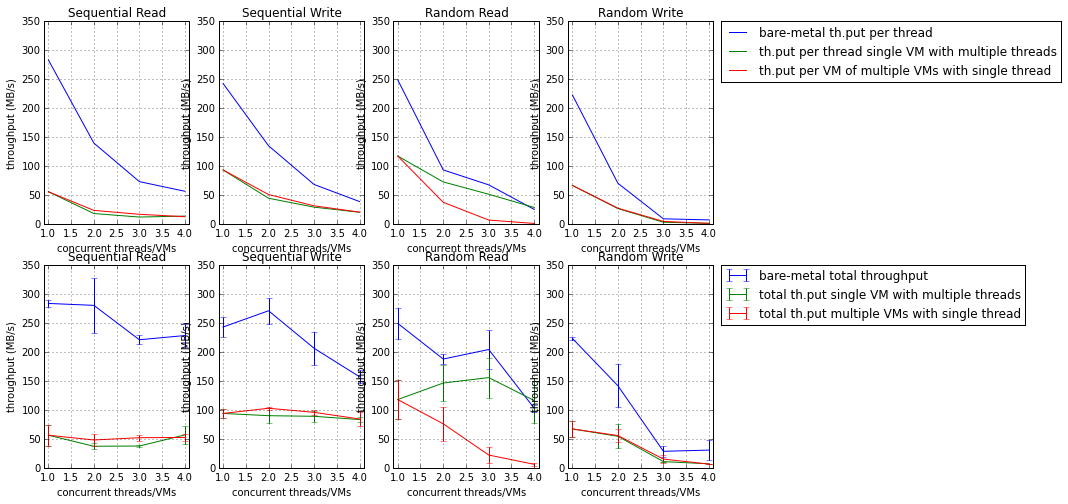
\includegraphics[scale=1]{throughput}

%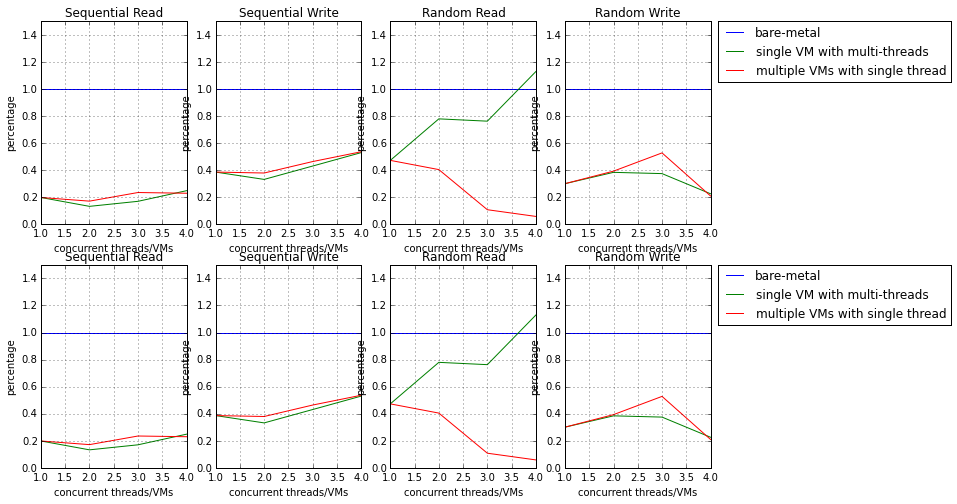
\includegraphics[scale=1]{nml_throughput}

\subsubsection{Jain Fairness Index}
%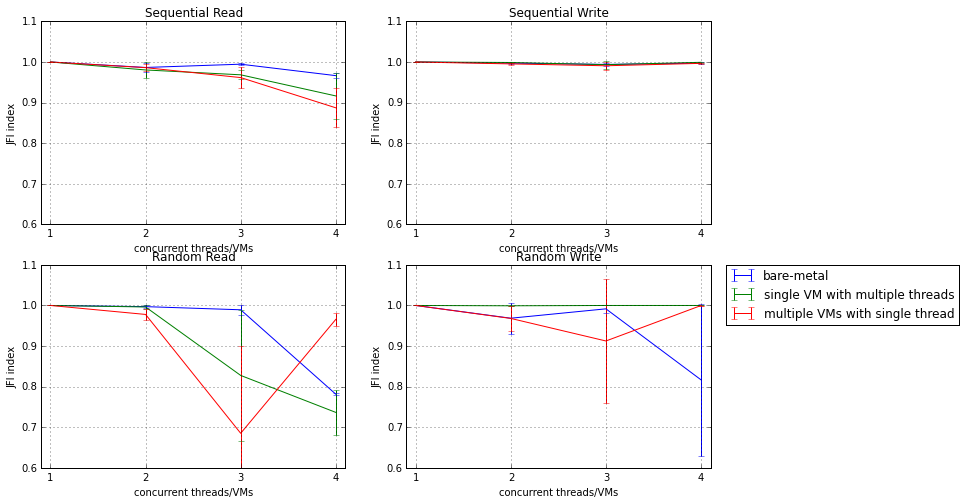
\includegraphics[scale=1]{JFI}

Jain Fairness Index (JFI) has a range from 0 to 1 which indicates the level of fairness between concurrent threads. If the threads receive equal partition of bandwidth, we would achieve index of 1. If only k of n flows receive equal bandwidth (and others get none), index is k/n. In the worst case, JFI has the index of 0. We plot some figures of JFI for the three scenarios with confident interval of 95\%. The figures show that threads have very equal throughput except the case of Random Read and Random Write. We notice the reader that the figures show value of JFI from 0.6 to 1.1 for a clear view on the JFI of the system. We observe from the data that in Random Read and Random Write test, JFI is low because one of thread receives very high throughput but others receive low (need to verify with different system and different test) 

\subsubsection{CPU vs. Disk utilization}

%\includegraphics[scale=1]{CPUutilization}

The figures above represent the aggregated time for all threads to finish and the aggregated actual time that the thread are using the CPU. Because the amount of transfered data was multiplied proportional to the number of threads/VMs joining the test, so we cannot see clearly the overhead between the three scenarios. The distance between the solid line and the dash line represent the amout of useless time that the thread has to wait to finish its reading/writing. With this idea in mind, in later tests, we will use the same amount of transfered data to best present the overhead in terms of CPU utilization and CPU waiting time. The idea to use fixed data size is to see the increasing overhead when parallelism level increases.

The figures suggest that for the same amount of data, the threads inside VMs occupied the CPU more time than the bare-metal to accomplish the tasks. There is not much different between the two virtualized scenarios: Single VM with multiple threads and multiple VM with single thread. CPU spending time is a very important metric since it represent how well the process use the allocated CPU slot. For the same amount of work unit, threads inside VM spend double the time that the same ones use inside the bare-metal environment.

In bare-metal environment, the common thought is that sequential write is always slower than sequential read. But in the case of virtualized environment, we can see that sequential write is better than sequential read. The "Sequential Write" CPU utilisation can explain for the better throughput of sequential write operator in virtualized environment: because the thread running time and CPU utilisation of sequential write is less than sequential thread so we have better throughput. (Why??? maybe need to look for the way hypervisor manage the storage)

The waiting time is increasing when there are more threads accessing disk in parallel. However, because the transfer volume is increase gradually proportional to the number of parallel threads, we can not see clearly the overhead when the number of concurrent threads increases. Later experiments should fix this and draw conclusion on the behaviors of the system when parallelism is increase. These figure also lack of the disk utilisation. When disk utilisation is the bottleneck, the thread running time and CPU spending time will also increase. In later experiment, we will extract also the disk utilisation to see how it affect on CPU spending time.

%\includegraphics[scale=1]{nml_CPUutilization}

To illustrate the overhead in CPU spending time and Thread Running Time incurred by the virtualization, we also plot the normalization of the CPU Spending Time and Thread Running Time figure using bare-metal data as baseline for comparison. The figures show that for the same amount of transfered data, VMs spend double the time using the CPU. They also spend more time waiting for CPU slot, about 2 to 6 times in comparing to the bare-metal. One of the reason may also due to the bottleneck at the hard disk. This one can be verified by comparing the disk utilisation of the bare-metal and the virtualized scenarios.

\subsubsection{IOPS}
%\includegraphics[scale=1]{IOPS}
\subsubsection{Latency}
%\includegraphics[scale=1]{Latency}


%%%%%%%%%%%%%%%%%%%%%%%%%%%%%%%%%%%%%%%%%%%%%%%%%%%%%%%%%%%%%%%%%%%%%





%%%%%%%%%%%%%%%%%%%%%%%%%%%%%%%%%%%%%%%%%%%%%%%%%%%%%%%%%%%%%%%%%%%%%
\section{Conclusion}
%%%%%%%%%%%%%%%%%%%%%%%%%%%%%%%%%%%%%%%%%%%%%%%%%%%%%%%%%%%%%%%%%%%%%



%%%%%%%%%%%%
% THIS PART IS FOR THE REFERENCE SECTION
%%%%%%%%%%%%
% \balance
% \bibliographystyle{abbrv}
% \bibliography{ref}

\end{document}
